\documentclass[12pt, a4paper]{article}
\usepackage{fancyvrb}
\usepackage{float}
\usepackage[left=2cm, right=2cm, top=2cm, bottom=2cm]{geometry}
\usepackage{graphicx}
\usepackage{xeCJK}

\renewcommand\arraystretch{1.1}
\setCJKmainfont[AutoFakeBold=1.5]{新細明體}

\title{
  Network Administration/System Administration\\
  (NTU CSIE, Spring 2024)\\
  Lab 5 - Docker \& Kubernetes
}
\author{\Large B12902110 呂承諺}

\begin{document}
  \maketitle
  \section*{Task 1}
  \begin{figure}[H]
    \centering
    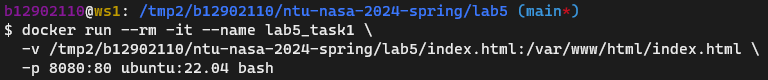
\includegraphics[width=\textwidth]{task1_docker_run.png}
  \end{figure}
  \begin{figure}[H]
    \centering
    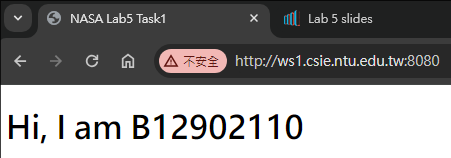
\includegraphics[width=0.5\textwidth]{task1_browser.png}
  \end{figure}

  \section*{Task 2}
  \verb|Dockerfile|:
\begin{Verbatim}[frame=single]
FROM ubuntu:22.04
RUN apt-get update && apt-get install -y nginx
COPY index.html /var/www/html/index.html
EXPOSE 80
ENTRYPOINT [ "nginx", "-g", "daemon off;" ]
\end{Verbatim}
  \begin{figure}[H]
   \centering
   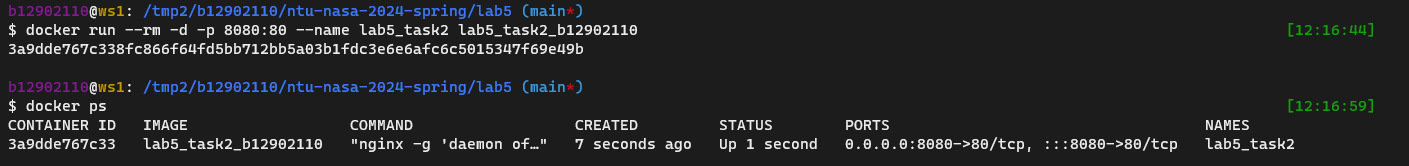
\includegraphics[width=\textwidth]{task2_docker.png}
  \end{figure}
  \begin{figure}[H]
   \centering
   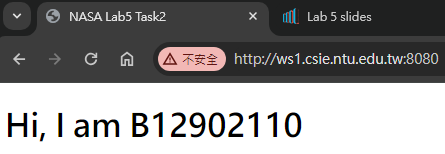
\includegraphics[width=0.5\textwidth]{task2_browser.png}
  \end{figure}

  \section*{Task 3}
  \begin{figure}[H]
   \centering
   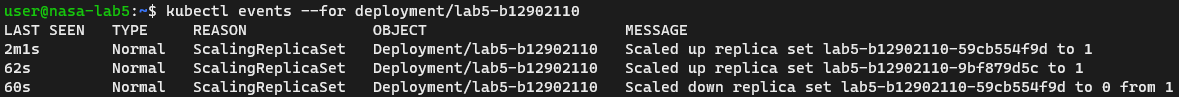
\includegraphics[width=\textwidth]{task3_kubectl_events.png}
  \end{figure}
  \begin{figure}[H]
   \centering
   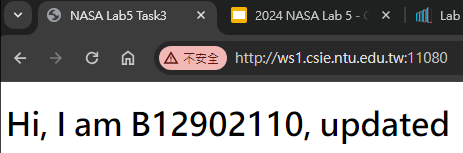
\includegraphics[width=0.5\textwidth]{task3_browser.png}
  \end{figure}
\end{document}
